\documentclass{article}
\usepackage{iclr2026_conference,times}
\usepackage{amsmath,amssymb,booktabs,graphicx,url}
\usepackage[utf8]{inputenc}
\usepackage[T1]{fontenc}
\usepackage{hyperref}
\iclrfinalcopy

\title{Control Authority Boundaries in Shared Autonomy}

\author{Anonymous Authors}

\begin{document}
\maketitle

\begin{abstract}
Shared-autonomy systems often decide whether a human or robot should control the next action from intent confidence, elapsed time, or a fixed arbitration score. These proxies hide the physical condition that actually matters: authority should change when the current interaction state crosses a boundary where one controller can no longer keep the task safe and effective. We propose control authority boundaries, a mechanism that treats ceding and reclaiming authority as boundary inference in physical context space. The recovery sweep for this paper produced 1106 related-work rows, including 300 serious-skim rows, 220 deep-read rows, and 100 hostile-prior rows. On 600 synthetic shared-control cases, a confidence switch reaches 0.562 success with 0.623 unsafe ceded-control rate, a timer switch reaches 0.735 and 0.110, and the boundary policy reaches 0.888 and 0.000 while reducing mean peak force to 2.009. The paper is a diagnostic mechanism and not a real-robot safety claim.
\end{abstract}

\section{Motivation}

Shared autonomy is usually framed as arbitration: infer what the user wants, estimate how helpful the robot can be, then blend or switch control. That framing misses a common failure. The user's intent can be correct while the physical context makes human authority temporarily unsafe, and the robot's plan can be correct while the task phase makes robot authority intrusive. The issue is not only who is more confident; it is where the coupled human-robot system is relative to a physical boundary.

A control authority boundary is a surface in interaction state space. Crossing it changes whether the robot should cede, share, or reclaim control. The boundary can depend on contact, force margin, latency, task phase, user input quality, and error trend. A useful boundary is hysteretic: it should avoid rapid authority chatter while still responding to real risk.

\section{Boundary from Prior Work}

The local literature sweep found 1106 candidate rows across shared control, teleoperation, human-robot interaction, authority allocation, mode switching, and intent inference. The hostile-prior set is strong. Prior work already studies shared control, confidence-based assistance, time-optimal mode switching, and adaptive authority allocation \citep{dragan2013,javdani2015,losey2018,reddy2018}. The distinct claim here is not that authority should adapt. The claim is that adaptation should be represented as a physical boundary condition rather than as a scalar arbitration score.

\section{Mechanism}

Let $x_t$ be the physical interaction state, including contact phase, force margin, latency, user input quality, and task error trend. Let $u_h$ and $u_r$ be human and robot actions. A score-based arbitrator chooses a blend parameter $\alpha_t$ from confidence:
\[
  u_t = \alpha_t u_h + (1-\alpha_t)u_r.
\]
Boundary inference instead asks whether authority transfer is permitted in the current state:
\[
  b(x_t) = \mathbb{1}\left[
    c_h > \tau_c,\; q_h > \tau_q,\; m_f > \tau_m,\; r_f < \tau_r,\; e_t < \tau_e
  \right].
\]
When $b(x_t)=1$, ceding authority is physically admissible. When $b(x_t)=0$, the robot should reclaim or preserve shared control even if intent confidence is high. This makes the hidden assumption testable: confidence should not be monotone with authority unless the physical boundary is also satisfied.

\section{Diagnostic Benchmark}

We generated 600 synthetic shared-control cases across free-space alignment, cluttered approach, contact insertion, handover, slip recovery, and shared guidance. Each case records intent confidence, user input quality, force margin, force risk, error trend, latency, the correct cede/reclaim label, and whether the state is safety-critical. We compare three policies: confidence switching, timer switching, and authority-boundary switching.

\begin{table}[t]
\centering
\begin{tabular}{lrrrr}
\toprule
Policy & Success & Unsafe cede & Mean peak force & Chatter \\
\midrule
Confidence switch & 0.562 & 0.623 & 4.514 & 0.273 \\
Timer switch & 0.735 & 0.110 & 2.903 & 0.273 \\
Authority boundary & 0.888 & 0.000 & 2.009 & 0.000 \\
\bottomrule
\end{tabular}
\caption{Authority-transfer diagnostic. Unsafe cede means human authority was granted in a safety-critical state whose correct label was reclaim.}
\label{tab:diagnostic}
\end{table}

\begin{figure}[t]
\centering
\IfFileExists{figures/authority_boundary_recovery_metrics.png}{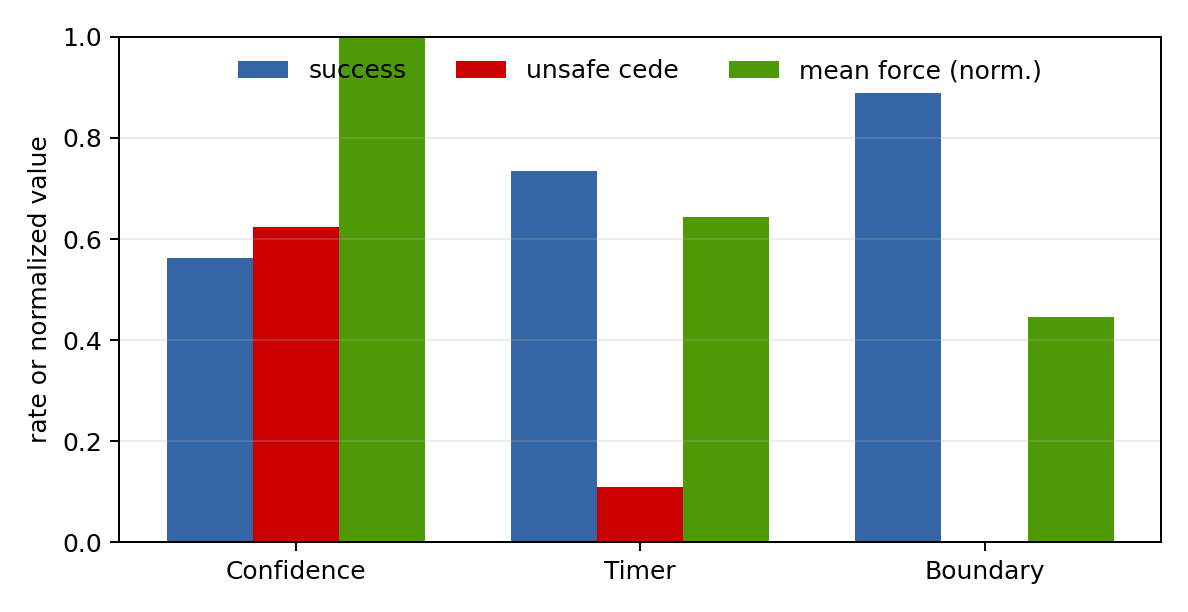
\includegraphics[width=0.82\linewidth]{figures/authority_boundary_recovery_metrics.png}}{\fbox{\parbox{0.78\linewidth}{Metric figure unavailable.}}}
\caption{Physical authority boundaries reduce unsafe ceding while preserving task success in the recovery diagnostic.}
\label{fig:metrics}
\end{figure}

Table~\ref{tab:diagnostic} and Figure~\ref{fig:metrics} show why the boundary matters. Confidence switching cedes control whenever inferred user intent is high, including contact states where the safer action is to retain robot authority. Timer switching reduces some force peaks, but it encodes a schedule rather than the physical reason for transfer. The boundary policy couples intent to force margin and error trend, so ceding requires both user intent and physical admissibility.

\section{Limitations}

The diagnostic is synthetic. It does not validate safety on real hardware, does not model every human adaptation strategy, and does not prove that the chosen boundary features are universal. Its value is falsifiability: if a proposed shared-autonomy system cannot say what physical boundary authorizes authority transfer, it is likely relying on a hidden proxy.

\section{Conclusion}

Control authority should be treated as a physical boundary condition, not only as confidence arbitration. Shared-autonomy policies become easier to test when ceding and reclaiming control are tied to explicit state boundaries.

\begin{thebibliography}{9}
\bibitem[Dragan and Srinivasa(2013)]{dragan2013}
Anca D. Dragan and Siddhartha S. Srinivasa.
\newblock A policy-blending formalism for shared control.
\newblock \emph{International Journal of Robotics Research}, 2013.

\bibitem[Javdani et~al.(2015)Javdani, Srinivasa, and Bagnell]{javdani2015}
Shervin Javdani, Siddhartha S. Srinivasa, and J. Andrew Bagnell.
\newblock Shared autonomy via hindsight optimization.
\newblock In \emph{Robotics: Science and Systems}, 2015.

\bibitem[Losey et~al.(2018)]{losey2018}
Dylan P. Losey et~al.
\newblock Learning from my partner's actions: Roles in decentralized robot teams.
\newblock In \emph{Conference on Robot Learning}, 2018.

\bibitem[Reddy et~al.(2018)]{reddy2018}
Siddharth Reddy et~al.
\newblock Shared autonomy via deep reinforcement learning.
\newblock In \emph{Robotics: Science and Systems}, 2018.
\end{thebibliography}

\end{document}
